%
%===============>>  ГРУППА 11-2 МОДУЛЬ 7  <<=============
%
\setmodule{7}

%BEGIN_FOLD % ====>>_____ Занятие 1 _____<<====
\begin{class}[number=1]
	\begin{listofex}
	\item %484557
	\begin{tasks}(1)
		\task Решите уравнение \( (2\sin x+\sqrt{3}) \cdot \sqrt{\cos x}=0 \)
		\task Найдите все корни этого уравнения, принадлежащие отрезку: \( \left[ \dfrac{3\pi}{2}; \dfrac{7\pi}{2} \right] \)
	\end{tasks}
	\item %501689
	\begin{tasks}(1)
		\task Решите уравнение \( 15^{\cos x}=3^{\cos x} \cdot 5^{\sin x} \)
		\task Найдите все корни этого уравнения, принадлежащие отрезку: \( \left[ 5\pi; \dfrac{13\pi}{2} \right]  \)
	\end{tasks}
	\item %505102
	\begin{tasks}(1)
		\task Решите уравнение \( 9^{\sin{x}}+9^{-\sin x}=\dfrac{10}{3} \)
		\task Найдите все корни этого уравнения, принадлежащие отрезку: \( \left[ -\dfrac{7\pi}{2}; -2\pi \right]  \)
	\end{tasks}
	\item %505236
	\begin{tasks}(1)
		\task Решите уравнение \( \left( \dfrac{2}{5} \right)^{\cos x}+ \left( \dfrac{5}{2} \right)^{\cos x}=2 \)
		\task Найдите все корни этого уравнения, принадлежащие отрезку: \( \left[ -3\pi;-\dfrac{3\pi}{2} \right]  \)
	\end{tasks}
	\item %505565
	\begin{tasks}(1)
		\task Решите уравнение \( \dfrac{3^{\cos x}}{9^{\cos^2x}}=4^{2\cos^2x-\cos x} \)
		\task Найдите все корни этого уравнения, принадлежащие отрезку: \( \left[ -\dfrac{3\pi}{2}; \dfrac{\pi}{6} \right]  \)
	\end{tasks}
	\item %501729
	\begin{tasks}(1)
		\task Решите уравнение \( (27^{\cos x})^{\sin x}=3^{\frac{3\cos x}{2}} \)
		\task Найдите все корни этого уравнения, принадлежащие отрезку: \( \left[ -\pi; \dfrac{\pi}{2} \right]  \)
	\end{tasks}
	\item %500192
	\begin{tasks}(1)
		\task Решите уравнение \( \left( \dfrac{1}{81} \right)^{\cos x}=9^{2\sin{2x}} \)
		\task Найдите все корни этого уравнения, принадлежащие отрезку: \( [-3\pi; -2\pi] \)
	\end{tasks}
	\end{listofex}
\end{class}
%END_FOLD

%BEGIN_FOLD % ====>>_____ Занятие 2 _____<<====
\begin{class}[number=2]
	\begin{listofex}
		\item Занятие 2
	\end{listofex}
\end{class}
%END_FOLD

%BEGIN_FOLD % ====>>_ Домашняя работа 1 _<<====
\begin{homework}[number=1]
	\begin{listofex}
		\item %525117
		\begin{tasks}(1)
			\task Решите уравнение: \( 2\log_2^2 (2\cos x) - 9 \log_2 (2\cos x) +4 = 0 \)
			\task Найдите все корни этого уравнения, принадлежащие отрезку: \( \left[ -2\pi; -\dfrac{\pi}{2} \right] \)
		\end{tasks}
		\item %500447
		\begin{tasks}(1)
			\task Решите уравнение: \( \log_2 (\cos x + \sin{2x} + 8) = 3 \)
			\task Найдите все корни этого уравнения, принадлежащие отрезку: \( \left[ \dfrac{3\pi}{2}; 3\pi \right] \)
		\end{tasks}
		\item %517438
		\begin{tasks}(1) 
			\task Решите уравнение: \( 8 \cdot 16^{\cos x} - 6 \cdot 4^{\cos x} + 1 = 0 \)
			\task Найдите все корни этого уравнения, принадлежащие отрезку: \( \left[ \dfrac{3\pi}{2}; 3 \pi \right] \)
		\end{tasks}
		\item %
		\begin{tasks}(1)
			\task Решите уравнение: \( 16^{\sin (\pi+x)}= \left( \dfrac{1}{2} \right)^{4\sin{(\frac{5\pi}{2}+x)}} \)
			\task Найдите все корни этого уравнения, принадлежащие отрезку: \( \left[ \dfrac{3\pi}{2}; 3\pi \right] \)
		\end{tasks}
		\item %523994
		\begin{tasks}(1)
			\task Решите уравнение: \( \dfrac{\log^2_2 (\sin x) + \log_2 (\sin{x})}{2\cos x - \sqrt{3}} = 0 \)
			\task Найдите все корни этого уравнения, принадлежащие отрезку: \( \left[ \dfrac{\pi}{2}; 2\pi \right] \)
		\end{tasks}
	\end{listofex}
\end{homework}
%END_FOLD

%BEGIN_FOLD % ====>>_____ Занятие 3 _____<<====
\begin{class}[number=3]
	\begin{listofex}
		\item Решите системы неравенств:
		\begin{tasks}(2)
			\task \( \begin{cases} 4x+9 \le 9x+4 \\ 1,7x \le 51 \end{cases} \)
			\task \( \begin{cases} (x+6)^2 < (x+4)^2 \\ 6x+13 > 5x-7 \end{cases} \)
			%\task \( \begin{cases}  \\  \end{cases} \)
			%\task \( \begin{cases}  \\  \end{cases} \)
		\end{tasks}
		\item Решите неравенства:
		\begin{tasks}(2)
			\task \( 10x^2+7x \le 0 \)
			\task \( 36x^2-25 > 0 \)
			\task \( x^2-19x+18 > 0 \)
			\task \( 2x^2-9x-5 < 0 \)
		\end{tasks}
		\item Решите двойное неравенство: \[ 3x^2-4x+3 \le 3x^2-5x+5 \le 2x^2-3x+4 \]
		\item Решите неравенства:
		\begin{tasks}(1)
			\task \( (3x^2-8x+4)(5x^2-8x-4) \le 0 \)
			\task \( (x+1)(x+2)(x+3)^2(x+4)^3 \le 0 \)
		\end{tasks}
		
		\item Решите систему неравенств: \[ \begin{cases} (2x^2+9x+4)(4x^2+9x+2)(9x^2+2x+4) \le 0 \\ (1-16x^2)(5x^2+2x)(4x^2+20x+25) > 0 \end{cases} \]
		\item Решите неравенство: \[ (16x^2+14x+3)(2x-1) > (8x^2-2x-1)(2x+1) \]
		
	\end{listofex}
\end{class}
%END_FOLD

%BEGIN_FOLD % ====>>_____ Занятие 4 _____<<====
\begin{class}[number=4]
	\begin{listofex}
		\item Решите неравенства:
		\begin{tasks}(2)
			\task \( (2x-3)(5x+2)>(2x-3)(5x -2) \)
			\task \( (x-7)(x^2-9x-25) \le 0 \)
		\end{tasks}
		\item Решите системы неравенств:
		\begin{tasks}(2)
			\task \( \begin{cases} 4x+9 \le 9x+4 \\ 1,7x \le 51 \end{cases} \)
			\task \( \begin{cases} 5x+8 \le 8+5 \\ 2,3x \le 46 \end{cases} \)
		\end{tasks}
		\item Решите неравенство: %Рациональное 11
		\[ \dfrac{2x^2-6x}{x-4} \le x \]
		\item Решите неравенства: %Шестаков 15 стр 131 ном 5(1 вар)
		\[ \dfrac{3x^2+7x+6}{3x^2+7x-6} > 0 \]
		\item Решите неравенство: %Рациональное 10
		\[ \dfrac{2x^2-2x+1}{2x-1} \le 1 \]
		\item Решите систему неравенств: %Шестаков 15 стр 131 ном 12(1 вар)
		\[ \begin{cases} \dfrac{36-25x^2}{36+25x^2} > 0 \\[10pt] \dfrac{5x^2-6x}{5x^2-6x+56} > 0 \end{cases} \]
		\item Решите неравенство: %Рациональное 12
		\[ \dfrac{(x-1)^2+4(x+1)^2}{2} \le \dfrac{(3x+1)^2}{4} \]
		\item Решите неравенство: %Рациональное 9
		\[ \left( \dfrac{10}{5x-21}+\dfrac{5x-21}{10} \right)^2 \le \dfrac{25}{4} \]
		
	\end{listofex}
\end{class}
%END_FOLD

%BEGIN_FOLD % ====>>_ Домашняя работа 2 _<<====
\begin{homework}[number=2]
	\begin{listofex}
		\item Решите неравенства: %Шестаков15 с102 н7 8 9 Б с105 30 31 32 Б
		\begin{tasks}(2)
			\task \( \dfrac{ 1+7x }{4  }>2x+1 \)
			\task \( \dfrac{ x }{ 5 }+\dfrac{ x+2 }{ 3 }\le \dfrac{ 4x+5 }{ 15 }-\dfrac{ 2 }{ 3 } \)
			\task \( (x-6)^2 \le (x-4)^2 \)
			\task \( x^2-17x+16 >0 \)
			\task \( 5x^2+9x-2<0 \)
			\task \( 6x^2+x-15 > 0 \)
			\task \( x+\dfrac{ 50 }{ x-7 } \le -8 \)
			\task \( \dfrac{ x-1 }{ x-3 }  \le 1+\dfrac{1  }{ x-2 } \)
		\end{tasks}
		\item Решите системы неравенств: %Шестаков15 с103 н11 12 Б
		\begin{tasks}(2)
			%\task \( \begin{cases} 5x+8 \le 8x+5 \\ 2,3x \le 46 \end{cases} \)
			\task \( \begin{cases} 3(2x+5)-2(3x+5)>5x \\ \dfrac{ 4 }{ 5 }x<1,25x+9 \end{cases} \)
			\task \( \begin{cases} \dfrac{ (x-6)^2 }{ 25-x^2 } > 0 \\ 6x-x^2 > 0 \end{cases} \)
		\end{tasks}
		%\item Решите неравенство: %Рациональное 1 МИМО
		%\[ \dfrac{x^2-2x+1}{(x+2)^2} + \dfrac{x^2+2x+1}{(x-3)^2} \le \dfrac{(2x^2-x+5)^2}{2(x+2)^2(x-3)^2} \]
	\end{listofex}
\end{homework}
%END_FOLD

%BEGIN_FOLD % ====>>_____ Занятие 5 _____<<====
\begin{class}[number=5]
		\begin{listofex}
		\item Решите неравенство: \( \dfrac{ 9 }{ (4x+5)^2 } - \dfrac{ 18 }{ 4x+5 } + 8 < 0 \).
	\end{listofex}
	\begin{definit}
		\[ |f(x)|<b \Leftrightarrow \begin{cases} f(x)<b \\ f(x) > -b, \end{cases} \qquad |f(x)|>b \Leftrightarrow \begin{cases} f(x)>b \\ f(x) < -b. \end{cases} \]
	\end{definit}
	\begin{listofex}[resume]
		\item Решите неравенства: %Шестаков какие-то
		\begin{tasks}
			\task \( |3x+4| > 5 \)
			\task \( |x^2-9x+14| \le 6 \)
			\task \( |x^2-4x-8| \le x-2 \)
			\task \( ||x^2+3x+2| - 1| > 1 \)
			
			%\task \( \begin{cases}  \\  \end{cases} \)
		\end{tasks}
		\item Решите неравенства: %Шестаков какие-то
		\begin{tasks}
			\task \( |x+2|+|x+7| \le 25 \)
			\task \( |x^2-6x|-3|2x-3| \le x^2+3x \)
		\end{tasks}
		\item Решите систему неравенств: \( \begin{cases} |2x^2-4x-11| > 5 \\ |x^2-5| \le 4 \end{cases} \)
	\end{listofex}
\end{class}
%END_FOLD

%BEGIN_FOLD % ====>>_____ Занятие 6 _____<<====
\begin{class}[number=6]
	\begin{listofex}
		\item Решите неравенства: %163 A 16-21
		\begin{tasks}(2)
			\task \( |2x^2-13| \ge 5 \)
			\task \( |x^2-10x|<24 \)
			%\task \( |2x^2-5x| \le 3 \)
			%\task \( |x^2-15x| > 54 \)
			\task \( |3x^2-10x| \ge 8 \)
			\task \( |x^2-2x-16|<8 \)
		\end{tasks}
		\item Решите неравенства: %откуда-то
		\begin{tasks}(2)
			\task \( |4x^2-12x+7| \ge 2x-3 \)
			\task \( |x^3+10x-20| \le x^3+20 \)
			\task \( \left| \dfrac{ 3x+5 }{ x+2 } \right| \ge 2 \)
			\task \( \left| \dfrac{ x^2-10x+9 }{ x^2-9 } \right| \ge 1 \)
		\end{tasks}
		\item Решите неравенства: %183 A 1 2
		\( |x+2|+|x+7| \le 25 \)
		%\task \( |x-4|+|x+8| < 36 \)
		\item Решите систему неравенств: %163 27A
		\[ \begin{cases} |2x-5| \ge 15 \\ |5x-2| \le 48 \end{cases} \]
	\end{listofex}
\end{class}
%END_FOLD

%BEGIN_FOLD % ====>>_ Домашняя работа 3 _<<====
\begin{homework}[number=3]
	\begin{listofex}
		\item Решите неравенства: %162 11-19 b
		\begin{tasks}(2)
			\task \( |4x^2+5x-6| \le 0 \)
			\task \( |6x^2-67x-678| < 0 \)
			%\task \( |x^2-13| < 12 \)
			%\task \( |2x^2-17| \le 15 \)
			\task \( |2x^2-5| \ge 3 \)
			%\task \( |x^2-5x|<6 \)
			\task \( |3x^2-5x| \le 2 \)
			%\task \( |x^2-20x|>96 \)
		\end{tasks}
		\item Решите неравенства: \( |x+3|+|x+9| \le 23 \). %183 1-2 b
		%\task \( |x-5|+|x+6|<33 \)
		
		\item %тригон кос
		\begin{minipage}[t]{\bodywidth}
			На рисунке изображен график функции \(f(x) =a \cos x +b\). Найдите \(b\).
		\end{minipage}
		\hspace{0.02\linewidth}
		\begin{minipage}[t]{\picwidth}
			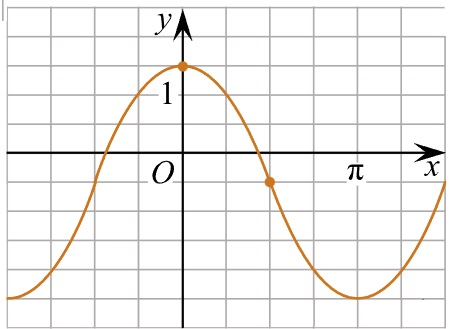
\includegraphics[align=t, width=\linewidth]{../pics/MECGERM6H3-1.jpg}
		\end{minipage}
		\item %тригон тг
		\begin{minipage}[t]{\bodywidth}
			На рисунке изображен график функции \(f(x) =a \tg x +b\). Найдите \(a\).
		\end{minipage}
		\hspace{0.02\linewidth}
		\begin{minipage}[t]{\picwidth}
			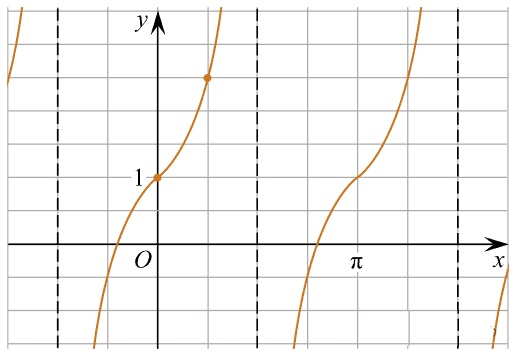
\includegraphics[align=t, width=\linewidth]{../pics/MECGERM6H3-2.jpg}
		\end{minipage}
		\item Найдите наименьшее значение функции \( y=4x-4 \ln(x+7)+6 \) на отрезке \( [-6,5;0] \). %3
		\item Найдите точку максимума функции \( y=\ln(x+5)^5-5x \) на отрезке. %12
		\item Найдите наибольшее значение функции \( y=12\cos x + 6\sqrt{3} x - 2 \sqrt{3} \pi + 6 \) на отрезке \( \left[ 0; \dfrac{ \pi }{ 2 } \right]  \).
	\end{listofex}
\end{homework}
%END_FOLD

%BEGIN_FOLD % ====>>_____ Занятие 7 _____<<====
\begin{class}[number=7]
	\begin{listofex}
		\item Решите неравенства:
		\begin{tasks}(2)
			\task \( \sqrt{x^2-144}\le5 \)
			\task \( \sqrt{3x^2-14x+51}\ge6 \)
			\task \( \sqrt{x^2-2x-15}<3 \)
		\end{tasks}
		\item Решите неравенства:
		\begin{tasks}(2)
			\task \( \sqrt[7]{7x-8} > -1 \)
			\task \( (7x-8)^{1/7} > -1 \)
		\end{tasks}
		\item Решите неравенства:
		\begin{tasks}(2)
			\task
			\(
			\left\{
			\begin{array}{l}
				\sqrt{x-3}\le2,\\
				\sqrt{12-x}\ge3.
			\end{array}
			\right.
			\)
			\task
			\(
			\left\{
			\begin{array}{l}
				\sqrt{x-3}\le5,\\
				(x^2-8x+15)^{1/15}\ge0.
			\end{array}
			\right.
			\)
		\end{tasks}
		\item Решите неравенства:
		\begin{tasks}(2)
			\task \( \sqrt{2x-1}<x-2 \)
			\task \( \sqrt{6x^2-x-1}\le x+1 \)
			\task \( \sqrt{5-2x}>7-3x \)
		\end{tasks}
	\end{listofex}
\end{class}
%END_FOLD

%BEGIN_FOLD % ====>>_ Проверочная работа _<<====
\begin{class}[number=8]
	\begin{listofex}
		\item Решите неравенства %192 a 3 4 20 21 22 24 23 25 ДАЛЬШЕ БРАТЬ С С193
		\begin{tasks}(2)
			\task \( \sqrt[13]{5x+9} \le 0 \)
			\task \( \sqrt[5]{-11-4x} < 0 \)
			\task \( \sqrt[5]{8x-x^2-17} < -1 \)
			\task \( \sqrt[16]{4x-4x^2} \ge 1 \)
			\task \( \sqrt[]{x^2-5x+1} > 5 \)
			\task \( \sqrt[28]{8x-x^2-15} < 1 \)
			\task \( (x^2-24x)^{\tfrac{1}{4}} \le 3 \)
			\task \( (6x-x^2)^{\tfrac{1}{3}} \le 2 \)
		\end{tasks}
		\item Решите неравенства: %222 a 2 4 5 6 c193 25 26 a
		\begin{tasks}(1)
			\task \( \sqrt[]{x^2-144} \le 6 \)
			\task \( \sqrt{x^2-2x-15} < 3 \)
			\task \( \sqrt[3]{x^4-4x^3+7x^2+3x+1} \le x+1 \)
			%\task \( \sqrt[]{x^4-2x+6} \ge x \)
			%\task \( \sqrt[]{5x^4-28x^2+16} \ge x^2+4 \)
			%\task \( \sqrt[]{x^2-17x-29} \ge 3|x+2| \)
		\end{tasks}
	\end{listofex}
\end{class}
%END_FOLD

%BEGIN_FOLD % ====>>_ Консультация cавель _<<====
\begin{consultation}
	\begin{listofex}
		\item
		\begin{minipage}[t]{\bodywidth}
			На рисунке изображён график функции \(f(x)=kx+b\). Найдите \(f(-9)\).
		\end{minipage}
		\hspace{0.02\linewidth}
		\begin{minipage}[t]{\picwidth}
			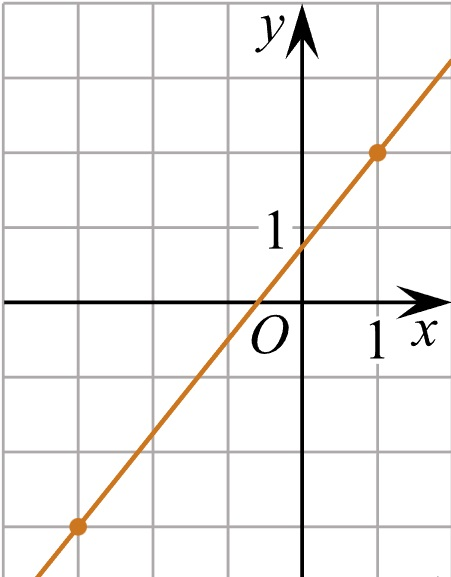
\includegraphics[align=t, width=\textwidth]{../pics/G101M4C4-1.jpg}
		\end{minipage}
		\item
		\begin{minipage}[t]{\bodywidth}
			На рисунке изображён график функции вида \(f(x)=ax^2+bx+c\), где числа \(a, b, c\) --- целые. Найдите значение \(f\left( -\mfrac{1}{1}{2} \right)\).
		\end{minipage}
		\hspace{0.02\linewidth}
		\begin{minipage}[t]{\picwidth}
			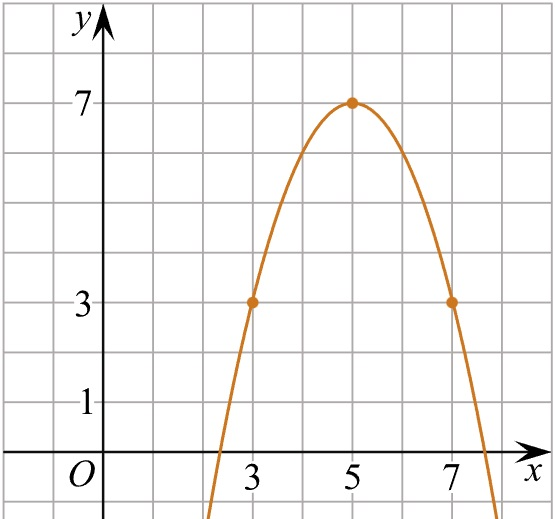
\includegraphics[align=t, width=\linewidth]{../pics/G101M4H2-5.jpg}
		\end{minipage}
		\item
		\begin{minipage}[t]{\bodywidth}
			На рисунке изображён график функции вида \[ f(x)=ax+|bx+c|+d, \] где числа \(a, b, c, d\) --- целые. Найдите корень уравнения \(ax+d=-15\).
		\end{minipage}
		\hspace{0.02\linewidth}
		\begin{minipage}[t]{\picwidth}
			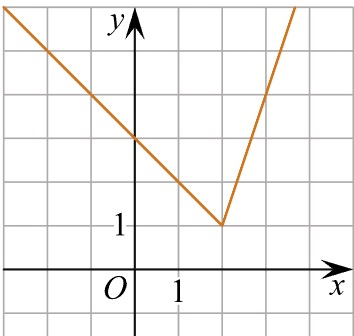
\includegraphics[align=t, width=\linewidth]{../pics/G101M4C5-7.jpg}
		\end{minipage}
		\item
		\begin{minipage}[t]{\bodywidth}
			На рисунке изображён график функции вида \[ f(x)=ax+|bx+c|+d, \] где числа \(a, b, c, d\) --- целые. Найдите корень уравнения \(bx+c=2\).
		\end{minipage}
		\hspace{0.02\linewidth}
		\begin{minipage}[t]{\picwidth}
			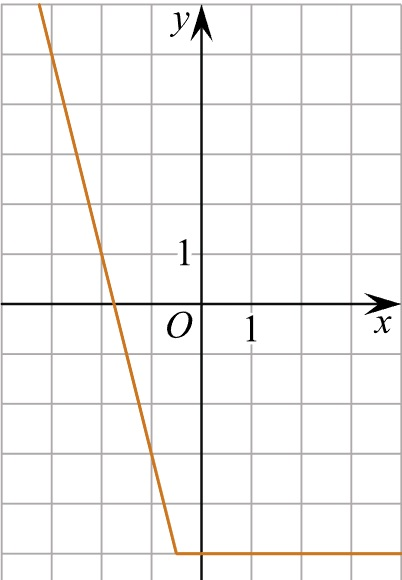
\includegraphics[align=t, width=\linewidth]{../pics/G101M4H2-6.jpg}
		\end{minipage}
		\item
		\begin{minipage}[t]{\bodywidth}
			На рисунке изображён график функции вида \[ f(x)=ax-|bx+c|+d, \] где числа \(a, b, c, d\) --- целые. Найдите корень уравнения \(ax+d=-2\).
		\end{minipage}
		\hspace{0.02\linewidth}
		\begin{minipage}[t]{\picwidth}
			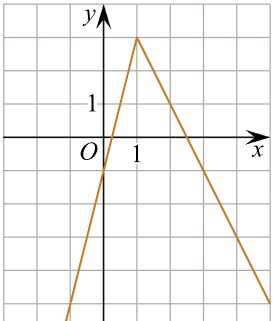
\includegraphics[align=t, width=\linewidth]{../pics/G101M4C6-8.jpg}
		\end{minipage}
		\item
		\begin{minipage}[t]{\bodywidth}
			На рисунке изображён график функции вида \[ f(x)=\dfrac{a}{x+b}+c, \] где числа \(a, b, c\) --- целые. Найдите значение \(x\), при котором \(f(x)=-5\).
		\end{minipage}
		\hspace{0.02\linewidth}
		\begin{minipage}[t]{\picwidth}
			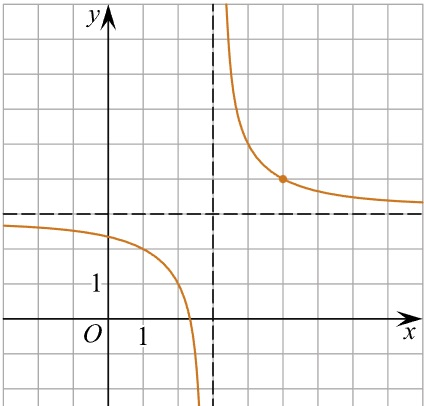
\includegraphics[align=t, width=\linewidth]{../pics/G101M4C6-2.jpg}
		\end{minipage}
		\item
		\begin{minipage}[t]{\bodywidth}
			На рисунке изображён график функции вида \[ f(x)=\dfrac{a}{x+b}+c, \] где числа \(a, b, c\) --- целые. Найдите значение \(x\), при котором \(f(x)=-5\).
		\end{minipage}
		\hspace{0.02\linewidth}
		\begin{minipage}[t]{\picwidth}
			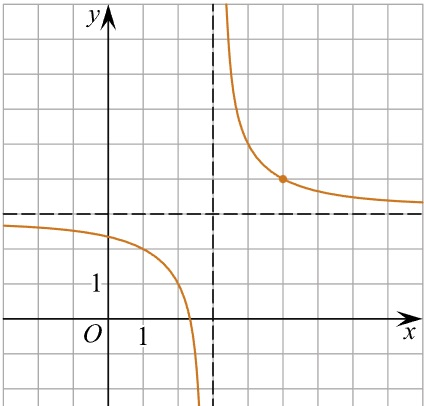
\includegraphics[align=t, width=\linewidth]{../pics/G101M4C6-2.jpg}
		\end{minipage}
		\item
		\begin{minipage}[t]{\bodywidth}
			На рисунке изображён график функции вида \[ f(x)=\dfrac{ax+b}{x+c}, \] где числа \(a, b, c\) --- целые. Найдите \(b\).
		\end{minipage}
		\hspace{0.02\linewidth}
		\begin{minipage}[t]{\picwidth}
			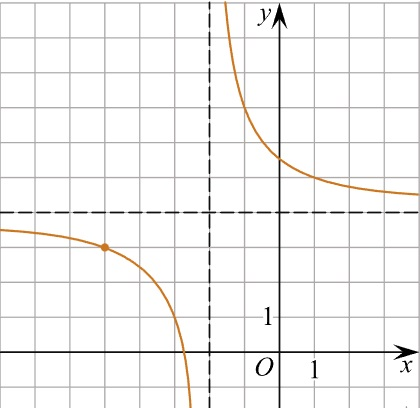
\includegraphics[align=t, width=\linewidth]{../pics/G101M4C6-5.jpg}
		\end{minipage}
		\item Найдите точку максимума функции \( y=x^3-48x+17 \).
		\item Найдите наименьшее значение функции \( y=x^3-27x \) на отрезке \( [0;4] \).
		\item Найдите наименьшее значение функции функции \( y=(x-8)e^{x-7} \) на отрезке \( [6;8] \).
		\item Найдите точку минимума функции \( y=(x+16)e^{x-16} \).
		\item Найдите наименьшее значение функции \( y=3x-\ln(x+3)^3 \) на отрезке \( [-2,5;0] \).
		\item Найдите наибольшее значение функции \( y=\ln (x+5)^5-5x \) на отрезке \( [-4,5;0] \).
		\item Найдите наибольшее значение функции \( y=12\cos x +6 \sqrt{3}x - 2 \sqrt{3} \pi +6 \) на отрезке \( \left[ 0; \dfrac{ \pi }{ 2 } \right]  \).
		\item Найдите наименьшее значение функции \( y=3+\dfrac{ 5\pi }{ 4 }-5x -5\sqrt{2}\cos x \) на отрезке \( \left[ 0; \dfrac{ \pi }{ 2 } \right]  \).
		\item Решите уравнения:
		\begin{tasks}(2)
			\task \( \log_{x^2}13=\log_{4-3x}13 \)
			\task \( (x+2)\log_{x+3}(x+4)=0 \)
			\task \( x^2+\log_7x+\log_7 \dfrac{ 7 }{  x}=50 \)
			\task \( \log_{15}x^4=\log_{15}(15x)^2 \)
		\end{tasks}
	\end{listofex}
\end{consultation}
%END_FOLD

%BEGIN_FOLD % ====>>_ Консультация коршун _<<====
\begin{consultation}
	\begin{listofex}
		\item На экзамен вынесено \(60\) вопросов, Андрей не выучил \(3\) из них. Найдите вероятность того, что ему попадется выученный вопрос.
		\item В среднем из \(1400\) садовых насосов, поступивших в продажу, \(7\) подтекают. Найдите вероятность того, что один случайно выбранный для контроля насос не подтекает.
		\item Фабрика выпускает сумки. В среднем \(8\) сумок из \(100\) имеют скрытые дефекты. Найдите вероятность того, что купленная сумка окажется без дефектов.
		\item При производстве в среднем на каждые \(2982\) исправных насоса приходится \(18\) неисправных. Найдите вероятность того, что случайно выбранный насос окажется неисправным.
		\item Какова вероятность того, что случайно выбранный телефонный номер оканчивается двумя чётными цифрами?
		\item Если шахматист \(A\) играет белыми фигурами, то он выигрывает у шахматиста \(B\) с вероятностью \(0,52\). Если \(A\) играет черными, то \(A\) выигрывает у \(B\) с вероятностью \(0,3\). Шахматисты \(A\) и \(B\) играют две партии, причём во второй партии меняют цвет фигур. Найдите вероятность того, что \(A\) выиграет оба раза.
		\item Вероятность того, что в случайный момент времени температура тела здорового человека окажется ниже чем \(36,8 \degree C\), равна \(0,81\). Найдите вероятность того, что в случайный момент времени у здорового человека температура окажется \(36,8 \degree C\) или выше.
		\item При изготовлении подшипников диаметром \(67\) мм вероятность того, что диаметр будет отличаться от заданного не больше, чем на \(0,01\) мм, равна \(0,965\). Найдите вероятность того, что случайный подшипник будет иметь диаметр меньше чем \(66,99\) мм или больше чем \(67,01\) мм.
		\item Симметричную монету бросают \(10\) раз. Во сколько раз вероятность события "выпадет ровно \(5\) орлов" больше вероятности события "выпадет ровно 4 орла"?
		\item В одном ресторане в г. Тамбове администратор предлагает гостям сыграть в "\textbf{Шеш-беш}": гость бросает одновременно две игральные кости. Если он выбросит комбинацию \(5\) и \(6\) очков хотя бы один раз из двух попыток, то получит комплимент от ресторана: чашку кофе или десерт бесплатно. Какова вероятность получить комплимент? Результат округлите до сотых.
		\item Игральную кость бросали до тех пор, пока сумма всех выпавших очков не превысила число \(3\). Какова вероятность того, что для этого потребовалось ровно два броска? Ответ округлите до сотых.
		\item Монету подбрасывают \(8\) раз. Найдите математическое ожидание количества выпавших орлов.
		\item Монету подбрасывают до тех пор, пока орёл не выпадет два раза (не обязательно подряд). Найдите математическое ожидание числа бросков.
		\item В торговом центре два одинаковых автомата продают кофе. Обслуживание автоматов происходит по вечерам после закрытия центра. Вероятность события "К вечеру в первом автомате закончится кофе" равна \(0,2\). Вероятность события "К вечеру в втором автомате закончится кофе" равна \(0,6\). Считая эти события независимыми, найдите математическое ожидание числа автоматов, в которых к вечеру закончится кофе.
		
	\end{listofex}
\end{consultation}
%END_FOLD

%BEGIN_FOLD % ====>>_ Консультация cавель _<<====
\begin{consultation}
	\begin{listofex}
		\item
		\begin{minipage}[t]{\bodywidth}
			На рисунке изображён график функции \(f(x)=kx+b\). Найдите \(f(-9)\).
		\end{minipage}
		\hspace{0.02\linewidth}
		\begin{minipage}[t]{\picwidth}
			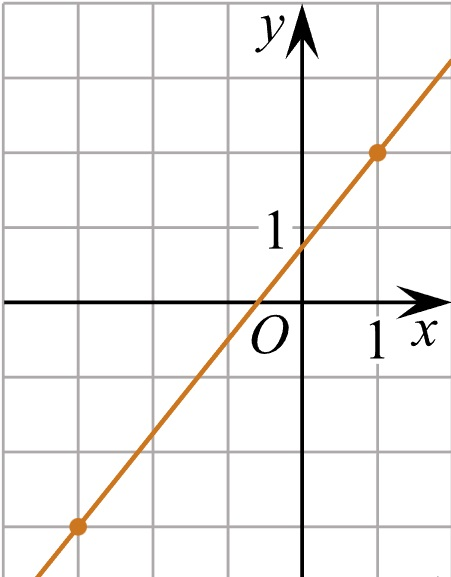
\includegraphics[align=t, width=\textwidth]{../pics/G101M4C4-1.jpg}
		\end{minipage}
		\item
		\begin{minipage}[t]{\bodywidth}
			На рисунке изображён график функции вида \(f(x)=ax^2+bx+c\), где числа \(a, b, c\) --- целые. Найдите значение \(f\left( -\mfrac{1}{1}{2} \right)\).
		\end{minipage}
		\hspace{0.02\linewidth}
		\begin{minipage}[t]{\picwidth}
			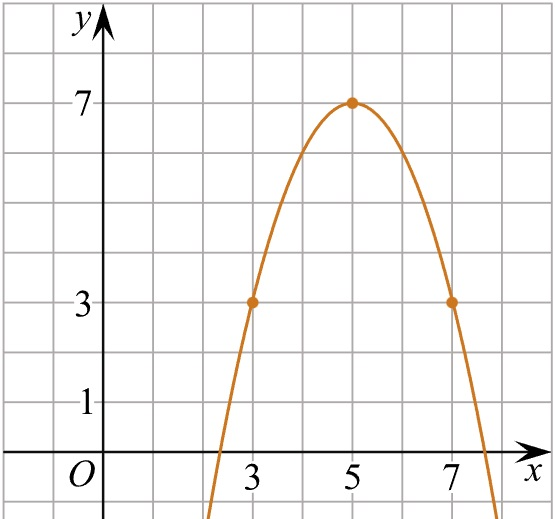
\includegraphics[align=t, width=\linewidth]{../pics/G101M4H2-5.jpg}
		\end{minipage}
		\item
		\begin{minipage}[t]{\bodywidth}
			На рисунке изображён график функции вида \[ f(x)=ax+|bx+c|+d, \] где числа \(a, b, c, d\) --- целые. Найдите корень уравнения \(ax+d=-15\).
		\end{minipage}
		\hspace{0.02\linewidth}
		\begin{minipage}[t]{\picwidth}
			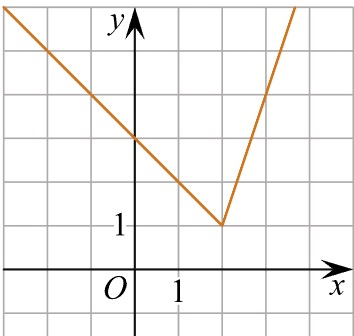
\includegraphics[align=t, width=\linewidth]{../pics/G101M4C5-7.jpg}
		\end{minipage}
		\item
		\begin{minipage}[t]{\bodywidth}
			На рисунке изображён график функции вида \[ f(x)=ax+|bx+c|+d, \] где числа \(a, b, c, d\) --- целые. Найдите корень уравнения \(bx+c=2\).
		\end{minipage}
		\hspace{0.02\linewidth}
		\begin{minipage}[t]{\picwidth}
			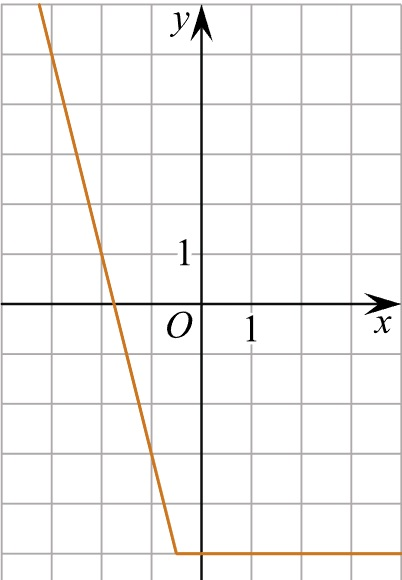
\includegraphics[align=t, width=\linewidth]{../pics/G101M4H2-6.jpg}
		\end{minipage}
		\item
		\begin{minipage}[t]{\bodywidth}
			На рисунке изображён график функции вида \[ f(x)=ax-|bx+c|+d, \] где числа \(a, b, c, d\) --- целые. Найдите корень уравнения \(ax+d=-2\).
		\end{minipage}
		\hspace{0.02\linewidth}
		\begin{minipage}[t]{\picwidth}
			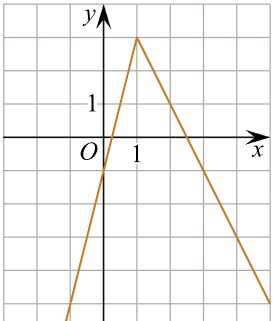
\includegraphics[align=t, width=\linewidth]{../pics/G101M4C6-8.jpg}
		\end{minipage}
		\item
		\begin{minipage}[t]{\bodywidth}
			На рисунке изображён график функции вида \[ f(x)=\dfrac{a}{x+b}+c, \] где числа \(a, b, c\) --- целые. Найдите значение \(x\), при котором \(f(x)=-5\).
		\end{minipage}
		\hspace{0.02\linewidth}
		\begin{minipage}[t]{\picwidth}
			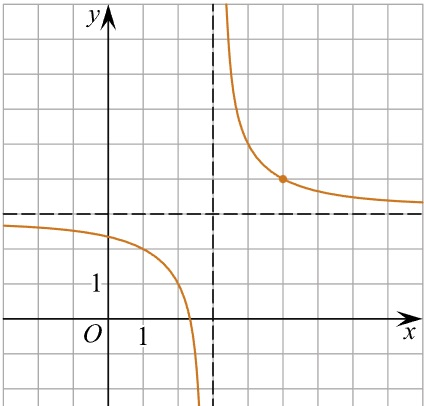
\includegraphics[align=t, width=\linewidth]{../pics/G101M4C6-2.jpg}
		\end{minipage}
		\item
		\begin{minipage}[t]{\bodywidth}
			На рисунке изображён график функции вида \[ f(x)=\dfrac{a}{x+b}+c, \] где числа \(a, b, c\) --- целые. Найдите значение \(x\), при котором \(f(x)=-5\).
		\end{minipage}
		\hspace{0.02\linewidth}
		\begin{minipage}[t]{\picwidth}
			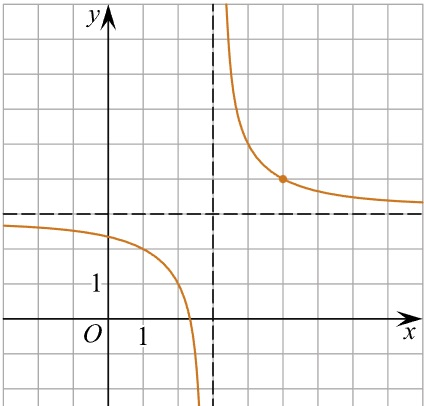
\includegraphics[align=t, width=\linewidth]{../pics/G101M4C6-2.jpg}
		\end{minipage}
		\item
		\begin{minipage}[t]{\bodywidth}
			На рисунке изображён график функции вида \[ f(x)=\dfrac{ax+b}{x+c}, \] где числа \(a, b, c\) --- целые. Найдите \(b\).
		\end{minipage}
		\hspace{0.02\linewidth}
		\begin{minipage}[t]{\picwidth}
			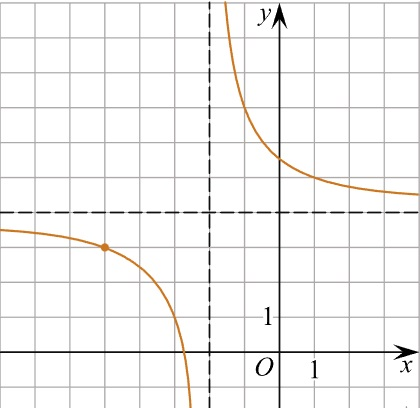
\includegraphics[align=t, width=\linewidth]{../pics/G101M4C6-5.jpg}
		\end{minipage}
		\item Найдите точку максимума функции \( y=x^3-48x+17 \).
		\item Найдите наименьшее значение функции \( y=x^3-27x \) на отрезке \( [0;4] \).
		\item Найдите наименьшее значение функции функции \( y=(x-8)e^{x-7} \) на отрезке \( [6;8] \).
		\item Найдите точку минимума функции \( y=(x+16)e^{x-16} \).
		\item Найдите наименьшее значение функции \( y=3x-\ln(x+3)^3 \) на отрезке \( [-2,5;0] \).
		\item Найдите наибольшее значение функции \( y=\ln (x+5)^5-5x \) на отрезке \( [-4,5;0] \).
		\item Найдите наибольшее значение функции \( y=12\cos x +6 \sqrt{3}x - 2 \sqrt{3} \pi +6 \) на отрезке \( \left[ 0; \dfrac{ \pi }{ 2 } \right]  \).
		\item Найдите наименьшее значение функции \( y=3+\dfrac{ 5\pi }{ 4 }-5x -5\sqrt{2}\cos x \) на отрезке \( \left[ 0; \dfrac{ \pi }{ 2 } \right]  \).
		\item Решите уравнения:
		\begin{tasks}(2)
			\task \( \log_{x^2}13=\log_{4-3x}13 \)
			\task \( (x+2)\log_{x+3}(x+4)=0 \)
			\task \( x^2+\log_7x+\log_7 \dfrac{ 7 }{  x}=50 \)
			\task \( \log_{15}x^4=\log_{15}(15x)^2 \)
		\end{tasks}
	\end{listofex}
\end{consultation}
%END_FOLD

%BEGIN_FOLD % ====>>_ Консультация коршун _<<====
\begin{consultation}
	\begin{listofex}
		\item На экзамен вынесено \(60\) вопросов, Андрей не выучил \(3\) из них. Найдите вероятность того, что ему попадется выученный вопрос.
		\item В среднем из \(1400\) садовых насосов, поступивших в продажу, \(7\) подтекают. Найдите вероятность того, что один случайно выбранный для контроля насос не подтекает.
		\item Фабрика выпускает сумки. В среднем \(8\) сумок из \(100\) имеют скрытые дефекты. Найдите вероятность того, что купленная сумка окажется без дефектов.
		\item При производстве в среднем на каждые \(2982\) исправных насоса приходится \(18\) неисправных. Найдите вероятность того, что случайно выбранный насос окажется неисправным.
		\item Какова вероятность того, что случайно выбранный телефонный номер оканчивается двумя чётными цифрами?
		\item Если шахматист \(A\) играет белыми фигурами, то он выигрывает у шахматиста \(B\) с вероятностью \(0,52\). Если \(A\) играет черными, то \(A\) выигрывает у \(B\) с вероятностью \(0,3\). Шахматисты \(A\) и \(B\) играют две партии, причём во второй партии меняют цвет фигур. Найдите вероятность того, что \(A\) выиграет оба раза.
		\item Вероятность того, что в случайный момент времени температура тела здорового человека окажется ниже чем \(36,8 \degree C\), равна \(0,81\). Найдите вероятность того, что в случайный момент времени у здорового человека температура окажется \(36,8 \degree C\) или выше.
		\item При изготовлении подшипников диаметром \(67\) мм вероятность того, что диаметр будет отличаться от заданного не больше, чем на \(0,01\) мм, равна \(0,965\). Найдите вероятность того, что случайный подшипник будет иметь диаметр меньше чем \(66,99\) мм или больше чем \(67,01\) мм.
		\item Симметричную монету бросают \(10\) раз. Во сколько раз вероятность события "выпадет ровно \(5\) орлов" больше вероятности события "выпадет ровно 4 орла"?
		\item В одном ресторане в г. Тамбове администратор предлагает гостям сыграть в "\textbf{Шеш-беш}": гость бросает одновременно две игральные кости. Если он выбросит комбинацию \(5\) и \(6\) очков хотя бы один раз из двух попыток, то получит комплимент от ресторана: чашку кофе или десерт бесплатно. Какова вероятность получить комплимент? Результат округлите до сотых.
		\item Игральную кость бросали до тех пор, пока сумма всех выпавших очков не превысила число \(3\). Какова вероятность того, что для этого потребовалось ровно два броска? Ответ округлите до сотых.
		\item Монету подбрасывают \(8\) раз. Найдите математическое ожидание количества выпавших орлов.
		\item Монету подбрасывают до тех пор, пока орёл не выпадет два раза (не обязательно подряд). Найдите математическое ожидание числа бросков.
		\item В торговом центре два одинаковых автомата продают кофе. Обслуживание автоматов происходит по вечерам после закрытия центра. Вероятность события "К вечеру в первом автомате закончится кофе" равна \(0,2\). Вероятность события "К вечеру в втором автомате закончится кофе" равна \(0,6\). Считая эти события независимыми, найдите математическое ожидание числа автоматов, в которых к вечеру закончится кофе.
		
	\end{listofex}
\end{consultation}
%END_FOLD

%BEGIN_FOLD % ====>>_ Доп. занятие _<<====
\begin{class}[number=доп. занятие]
	\begin{listofex}
		\item Найдите все значения параметра \( a \), при каждом из которых уравнение
		\[ (a-2)x^2-2(a-1)x+3=0 \]
		имеет единственный корень.
		\item При каких значениях параметра \( a \) уравнение
		\[ (a-2)x^2-4ax+a-1=0 \]
		имеет два корня разных знаков?
		\item При каких значениях параметра \( a \) уравнение
		\[ (a^2-9)x^2-(2a^2+5a-9)x+a+3=0 \]
		имеет два корня разных знаков?
		\item Найдите все значения параметра \( a \), при каждом из которых уравнение
		\[ x^2-2(a^2-4a+1)x+4=0 \]
		имеет два различных отрицательных корня.
		\item При каких значениях параметра \( a \) уравнение
		\[ x^2-(a+1)|x|+a=0 \]
		имеет три решения?
		\item При каких значениях параметра \( a \) уравнение
		\[ x^4-(3a-1)x^2+2a^2-a=0 \]
		имеет два решения?
	\end{listofex}
	\newpage
	\title{Домашняя работа}
	\begin{listofex}
		\item Найдите все значения параметра \( a \), при каждом из которых уравнение
		\[ (a-4)x^2-3(a+1)x+1=0 \]
		\item При каких значениях параметра \( a \) уравнение
		\[ (a+2)x^2-5ax+a-3=0 \]
		имеет два корня разных знаков?
		\item Найдите все значения параметра \( a \), при каждом из которых уравнение
		\[ x^2+2(a^2-6a-3)x+16=0 \]
		имеет два различных отрицательных корня.
	\end{listofex}
\end{class}